% Project Activity 2 report — compile with: latexmk -pdf main.tex   (figures: python3 make_figures.py)
\documentclass[10pt,a4paper,twocolumn]{article}

\usepackage[T1]{fontenc}
\usepackage{lmodern}
\usepackage[margin=1.35cm,top=1.15cm,bottom=1.3cm]{geometry}
\usepackage{amsmath}
\usepackage{graphicx}
\graphicspath{{figures/}}
\usepackage{booktabs}
\usepackage{tabularx}
\usepackage{array}
\usepackage{enumitem}
\usepackage[font=small,labelfont=bf,skip=2pt]{caption}
\usepackage{titlesec}
\usepackage{xcolor}
\usepackage[hidelinks]{hyperref}

\setlength{\columnsep}{0.55cm}
\titleformat{\section}{\normalsize\bfseries}{\thesection.}{0.4em}{}
\titlespacing*{\section}{0pt}{4pt}{1.5pt}
\setlist{nosep,leftmargin=1.2em,topsep=1pt}
\setlength{\parindent}{0pt}
\setlength{\parskip}{2pt}
\setlength{\textfloatsep}{5pt}
\setlength{\intextsep}{4pt}
\setlength{\floatsep}{4pt}
\setlength{\dbltextfloatsep}{5pt}
\setlength{\dblfloatsep}{4pt}
\renewcommand{\arraystretch}{1.05}
\newcolumntype{Y}{>{\raggedright\arraybackslash}X}
\newcommand{\hl}[1]{\textbf{#1}}

\begin{document}

\twocolumn[{
\begin{center}
{\large\bfseries Project Activity 2 Report: Baseline CNN for Fine-Grained Vehicle Classification}\\[2pt]
\small Introduction to AI Programming, Fall 2026 --- Project~1, Activity~2\\
Team: 20230906 Heeseon Yoo \quad 20230613 Donghyun Shin \quad 20230673 Seojin Han \quad 20230497 Hyeonil Cho\\
Dataset: \url{https://github.com/faezetta/VMMRdb} \quad Code: \href{https://github.com/heeseon28/intro_ai_project1/tree/main/task2}{\texttt{github.com/heeseon28/intro\_ai\_project1/tree/main/task2}}
\end{center}
\vspace{2pt}
}]

% ------------------------------------------------------------------ 1
\section{Dataset and Data Preparation}
We use the 50-class subset of VMMRdb \cite{vmmr} fixed in Activity~1: the 5 largest make-model classes of 10 makes
(production years merged), i.e.\ a \hl{50-way fine-grained make-model classification} task.
\begin{itemize}
  \item \hl{Splits}: 118,471 images after removing exact duplicates, split once with per-class stratification
  into \hl{82,929 train / 17,771 validation / 17,771 test} (70/15/15). Identical (MD5) images never cross splits.
  The split CSVs are versioned with SHA-256 hashes so that all later experiments reuse them.
  The \hl{test set is reserved} and was not used.
  \item \hl{Imbalance}: training images per class range from 184 (Jeep Patriot) to 4,805 (Honda Civic), a 26$\times$ gap.
  \item \hl{Preprocessing} (train and validation identically): RGB conversion, resize to 224$\times$224, tensor conversion,
  normalization with mean $=$ std $=0.5$ per channel. No augmentation.
\end{itemize}

% ------------------------------------------------------------------ 2
\section{Model and Training Configuration}
\begin{table}[h]
\centering\small
\caption{Baseline configuration (recorded in \texttt{config.json}).}\label{tab:cfg}
\footnotesize
\begin{tabularx}{\linewidth}{@{}l Y@{}}
\toprule
Architecture & ResNet-18 \cite{resnet} (torchvision), FC 512$\rightarrow$50, 11.2M params \\
Initialization & random (\texttt{weights=None}), no pre-training \\
Image size & 224$\times$224 RGB \\
Batch size / epochs & 64 / 12 (fixed, no early stopping) \\
Optimizer & Adam, learning rate $3\times10^{-4}$, no weight decay, no LR schedule \\
Loss & standard (unweighted) cross-entropy \\
Not used & augmentation, transfer learning, re-weighting/sampling, special losses \\
Checkpoint & epoch with the highest validation macro-F1 \\
Reproducibility & seed 0, FP32, deterministic cuDNN (bit-exact only on the same hardware) \\
Hardware & run A: GPU slice, 3.1\,min/epoch; run B: CPU, 106\,min/epoch \\
\bottomrule
\end{tabularx}
\end{table}

% ------------------------------------------------------------------ 3
\section{Training and Validation Performance}
Because the classes are imbalanced, we report \hl{macro-F1} (mean of per-class F1) and balanced accuracy
(mean per-class recall) in addition to accuracy. Table~\ref{tab:res} re-evaluates the selected checkpoint on both splits.
To check that the baseline is a reliable reference, the same code, split and seed were run twice by different
members on different hardware (run A: GPU, run B: CPU).

\begin{table}[h]
\centering\small
\caption{Performance of the selected checkpoint. Run A (epoch 12) is the reported baseline; run B (epoch 10) is an independent re-run.}\label{tab:res}
\begin{tabular}{@{}llrrrr@{}}
\toprule
Run & Split & Loss & Accuracy & Macro-F1 & Bal.\ acc. \\
\midrule
A & Train      & 0.109 & 96.4\% & 95.6\% & 95.7\% \\
A & Validation & 0.984 & \hl{77.0\%} & \hl{73.5\%} & 72.4\% \\
\midrule
B & Train      & 0.136 & 95.5\% & 94.5\% & 94.5\% \\
B & Validation & 0.920 & 77.1\% & 73.2\% & 72.8\% \\
\bottomrule
\end{tabular}
\end{table}

\begin{figure}[h]
\centering
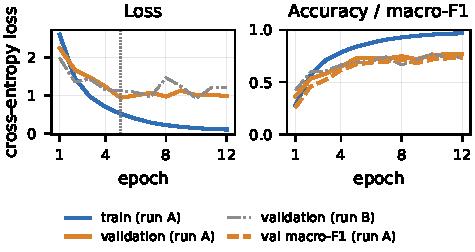
\includegraphics[width=\linewidth]{curves.pdf}
\caption{Learning curves of run A, with run B's validation curves (grey). Train values are averaged during each epoch's
updates; the dotted line marks run A's minimum validation loss (epoch 5).}\label{fig:curves}
\end{figure}

\hl{Q1: How well does the baseline classify the dataset?} About three of four validation images are classified
correctly (chance: 2\%), but macro-F1 is 3.6\,pp below accuracy and per-class F1 ranges from 0.39 to 0.93 (median 0.77):
performance is uneven across classes. The result is \hl{reproducible}: the two runs differ by 0.1\,pp in accuracy and
0.2\,pp in macro-F1, and their per-class F1 scores correlate at 0.92, so this baseline is a stable reference for later comparisons.

\hl{Overfitting, not underfitting.} Training accuracy reaches 96.4\% while validation accuracy is 77.0\%
(\hl{19.3\,pp gap}; run B: 18.4\,pp). In run A the validation loss stops improving after epoch 5 (0.94) and then
oscillates between 0.94 and 1.13, while the training loss keeps falling to 0.10 (Fig.~\ref{fig:curves}). The model fits
the training set far better than unseen images; it is not underfitting, since training accuracy is near 100\%.
Validation performance is also \hl{unstable without an LR schedule}: in run B, validation accuracy drops from 74.1\% to
66.4\% between epochs 7 and 8, and from 77.1\% (epoch 10) to 73.6\% at the last epoch. Longer training alone is therefore
unlikely to help, and the checkpoint must be chosen on the validation set. This choice makes the validation numbers slightly
optimistic, which is why the untouched test set is kept for the final, unbiased comparison.

% ------------------------------------------------------------------ 4
\begin{figure*}[t]
\centering
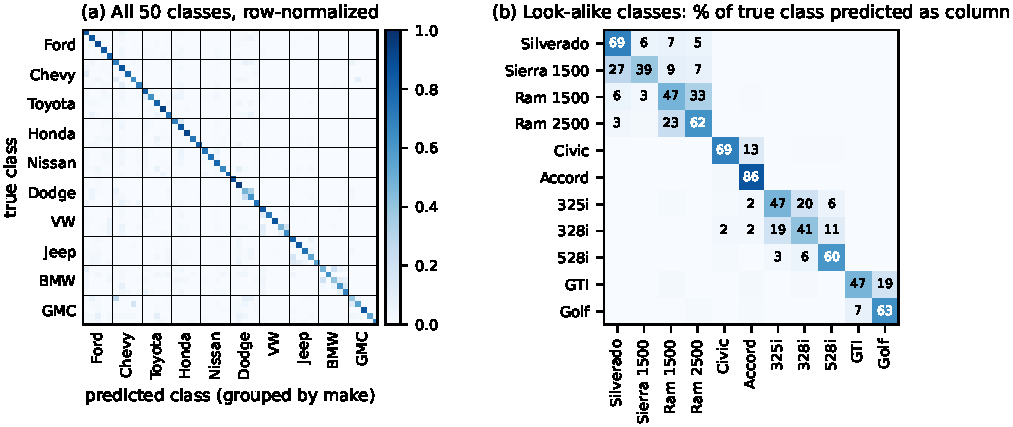
\includegraphics[width=0.84\textwidth]{confusion.pdf}
\caption{Validation confusion matrix. (a) All classes, ordered by make; off-diagonal mass is spread across makes.
(b) Look-alike classes; each number is the \% of a true class (row) predicted as the column class.}\label{fig:cm}
\end{figure*}

\begin{figure*}[t]
\centering
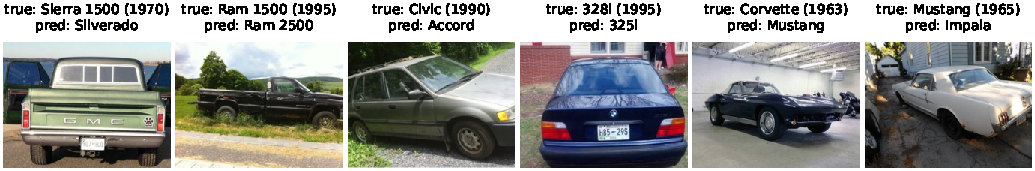
\includegraphics[width=0.88\textwidth]{errors.pdf}
\caption{Misclassified validation images for the main confusion pairs (first error of each pair in file order, not hand-picked).}\label{fig:err}
\end{figure*}

\section{Confusion Matrix and Difficult Classes}
\begin{table}[h]
\centering\small
\caption{Lowest-F1 classes, their training size, and their most frequent wrong prediction (\% of the class).}\label{tab:hard}
\begin{tabular}{@{}lrrl@{}}
\toprule
Class & $n_\text{train}$ & F1 & Most confused with \\
\midrule
Dodge Ram 1500   & 1,046 & 0.39 & Ram 2500 (33\%) \\
GMC Sierra 1500  & 1,124 & 0.42 & Chevy Silverado (27\%) \\
BMW 328i         &   594 & 0.45 & BMW 325i (19\%) \\
Dodge Ram 2500   &   867 & 0.45 & Ram 1500 (23\%) \\
BMW 528i         &   319 & 0.50 & BMW 530i (16\%) \\
VW Golf          &   330 & 0.52 & VW Jetta (9\%) \\
Jeep Cherokee    &   775 & 0.53 & Grand Cherokee (16\%) \\
\bottomrule
\end{tabular}
\end{table}

\hl{Q2: Which classes or images are difficult?} (Fig.~\ref{fig:cm}, Table~\ref{tab:hard}, Fig.~\ref{fig:err}).
The same classes are hardest in both runs (328i, Ram 1500, Sierra, Golf, Cherokee and Ram 2500 are in both bottom-six lists).
\begin{itemize}
  \item \hl{Look-alike pairs dominate the hardest classes}, as predicted in Activity~1:
  badge-engineered twins (Sierra$\rightarrow$Silverado 27\%), size variants of one truck (Ram 1500$\leftrightarrow$2500),
  and trims of one series (328i$\rightarrow$325i 19\%, GTI$\rightarrow$Golf 19\%). The largest single error count is
  Civic$\rightarrow$Accord (133 images), two similar sedans of the same make.
  \item \hl{Most errors cross makes}: of the 23.0\% validation error, \hl{16.8\,pp (73\%) go to a different make}
  and only 6.1\,pp stay within the correct make. Typical cross-make errors share a body type
  (Silverado$\rightarrow$Ram 1500, Corvette$\rightarrow$Mustang, Altima$\rightarrow$Accord). This suggests that the
  scratch-trained CNN relies mainly on the global silhouette rather than on small make cues such as emblems and grilles
  (to be checked with Grad-CAM in the next activity).
  \item \hl{Visual distinctiveness matters more than class size.} Larger classes tend to score higher
  (correlation of $\log n_\text{train}$ with F1: 0.44), and small classes are weak (528i 0.50, Golf 0.52, Patriot 0.65).
  But the two worst classes have over 1,000 training images, while the best ones have unique shapes
  (Odyssey 0.93, Grand Caravan 0.92, Beetle 0.91).
  \item \hl{Difficult images: old and rare generations.} Merging years mixes several generations in one class.
  Validation accuracy is 59.5\% for cars built before 1990, 72.3\% for the 1990s, and 81.1\% for the 2000s
  (the dominant decade), but drops to 68.2\% from 2010. Classic cars are often mistaken for other classics
  (1960s Mustang$\rightarrow$Impala, 1963 Corvette$\rightarrow$Mustang; Fig.~\ref{fig:err}).
\end{itemize}

% ------------------------------------------------------------------ 5
\section{Directions for Improvement}
\hl{Q3: What should we investigate next?} Each change will be tested on the same splits, with the same metrics, and with one change at a time against this baseline.
\begin{enumerate}[leftmargin=1.4em]
  \item \hl{Reduce overfitting} (19.3\,pp gap): data augmentation (random crop, flip, colour jitter),
  weight decay, and a learning-rate schedule with early stopping on validation macro-F1.
  \item \hl{Transfer learning}: ImageNet-pre-trained weights should provide generic shape and part features
  that 82k images cannot teach from scratch. As a reference upper bound, a separate run on the same splits with pre-training,
  augmentation, AdamW and a cosine schedule reached $94.2\pm0.1\%$ validation accuracy over 3 seeds. Because it changes several
  factors at once, it does not isolate the effect of pre-training; the controlled one-change experiments above will.
  \item \hl{Use the class hierarchy} (our Activity~1 hypotheses): since 73\% of errors cross makes, a make- or body-type-level
  first stage could remove many of them in the scratch setting. We will check whether this gain survives with pre-training.
  \item \hl{Target look-alike pairs}: aspect-preserving resize and a larger input size to keep emblem and grille detail.
  Class-balanced loss \cite{cbloss} for the small classes (Patriot, 528i, Golf).
  \item \hl{Reliability}: repeat each setting with 3 seeds and report mean $\pm$ std (runs A and B used the same seed, so they
  measure hardware/run variation, not seed variation). The test set is used only for the final comparison.
\end{enumerate}

% ------------------------------------------------------------------ 6
\section{Code and Reproduction}
\texttt{bash task2/run\_task2.sh -{}-data-root <VMMRdb> -{}-device cuda} trains and evaluates the baseline
(\texttt{task2/train\_baseline.py}) and writes the configuration with split and source hashes, the epoch history, metrics,
confusion matrix, per-class scores and predictions to \texttt{result\_task2/<run>/}. The submitted archive contains the code,
split files, both result folders (run A: \texttt{baseline\_seed0\_DonghyunShin}, run B: \texttt{baseline\_seed0\_Hyeonil\_Cho})
and a \texttt{README.md} with setup and run instructions.
\textit{Limitations}: one seed; near-duplicate images were not audited. Run B's recorded hashes differ from run A's only
because Windows converted line endings (contents verified identical).

{\footnotesize
\begin{thebibliography}{9}\setlength{\itemsep}{0pt}
\bibitem{vmmr} F.~Tafazzoli, H.~Frigui, K.~Nishiyama, ``A Large and Diverse Dataset for Improved Vehicle Make and Model Recognition,'' \textit{CVPR Workshops}, 2017.
\bibitem{resnet} K.~He, X.~Zhang, S.~Ren, J.~Sun, ``Deep Residual Learning for Image Recognition,'' \textit{CVPR}, 2016.
\bibitem{cbloss} Y.~Cui, M.~Jia, T.-Y.~Lin, Y.~Song, S.~Belongie, ``Class-Balanced Loss Based on Effective Number of Samples,'' \textit{CVPR}, 2019.
\end{thebibliography}
}

\end{document}
